\loesung{
\label{ex_sol:LIME_implementation}

The code for this exercise can be found in \texttt{sol\_lime.py} for Python or \texttt{sol\_lime.R} for R.

\begin{enumerate}[a)]
\item Inspect Implemented Functions

\lstinputlisting[firstline=1,lastline=84]{"rsrc/helper_functions_lime.R"}

Example: 
\lstinputlisting{"rsrc/data_lime.R"}
\lstinputlisting[firstline=6,lastline=11]{"rsrc/helper_functions_plot_lime.R"}

\begin{center}
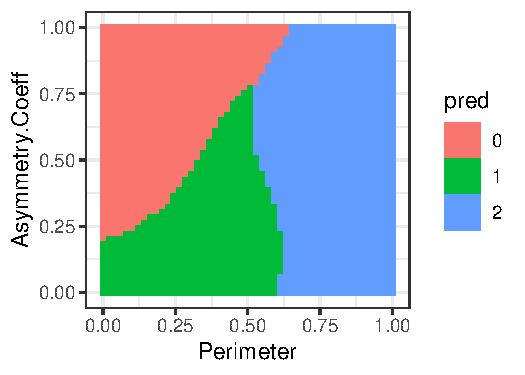
\includegraphics[width=\maxwidth]{figure/helper_functions_plot_lime.pdf}
\end{center}

\item Sample Points
\lstinputlisting[firstline=87,lastline=110]{"rsrc/helper_functions_lime.R"}

Example:
\lstinputlisting[firstline=5,lastline=9]{"rsrc/sample_points_plot_lime.R"}

\begin{center}
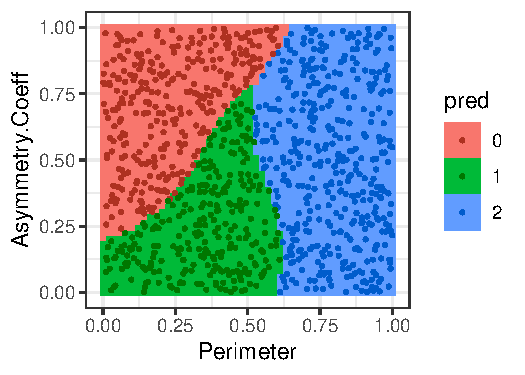
\includegraphics[width=\maxwidth]{figure/sample_points_plot_lime.pdf}
\end{center}

\item Weight Points
\lstinputlisting[firstline=114,lastline=140]{"rsrc/helper_functions_lime.R"}

Example:
\lstinputlisting[firstline=5,lastline=10]{"rsrc/weight_points_plot_lime.R"}

\begin{center}
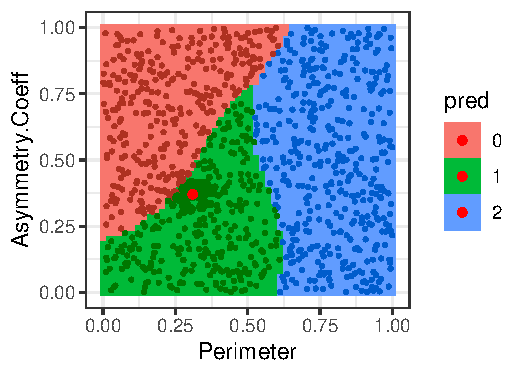
\includegraphics[width=\maxwidth]{figure/weight_points_plot_lime.pdf}
\end{center}

\item Fit Local Surrogate
\lstinputlisting[firstline=143,lastline=158]{"rsrc/helper_functions_lime.R"}

Example:
\lstinputlisting[firstline=5,lastline=22]{"rsrc/fit_explainer_model_plot_lime.R"}
\begin{center}
  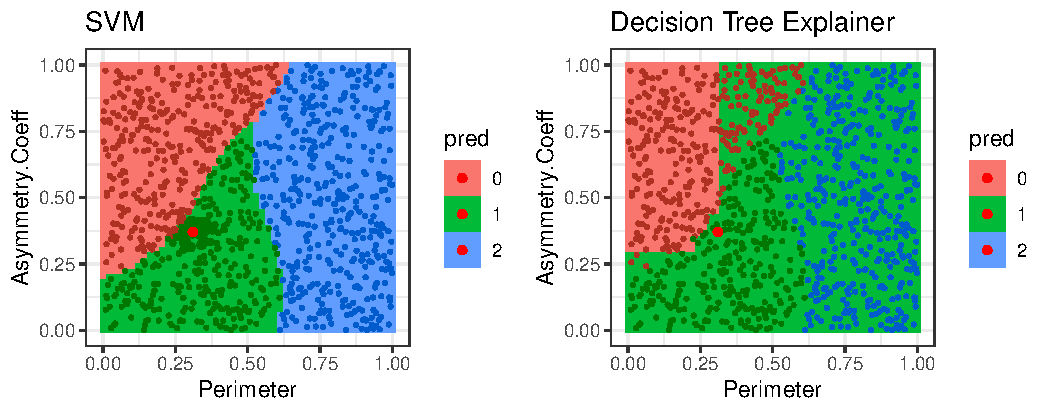
\includegraphics[width=\maxwidth]{figure/fit_explainer_model_plot_lime.pdf}
\end{center}

What could be problematic with a decision tree as the surrogate model?
\begin{itemize}
  \item Decision trees produce piecewise constant predictions, so they cannot capture smooth decision boundaries well. The local approximation may appear ``blocky'' compared to the original model.
  \item The tree depth (complexity) must be chosen carefully: a shallow tree is easy to interpret but may be too coarse; a deep tree fits the local data better but becomes harder to interpret, defeating the purpose of LIME.
  \item The surrogate model is fitted on sampled data that covers the entire feature space (not just the local neighborhood). The proximity weights help focus on the neighborhood, but far-away points with small weights can still influence the tree splits.
\end{itemize}



\end{enumerate}
}